% Figure A3: Figure 6b per act at 100M, and Figure 6c per model size. Drawn by dramatis scripts/paper_fig.py (make figures).
\begin{figure}[tbp]
  \centering
  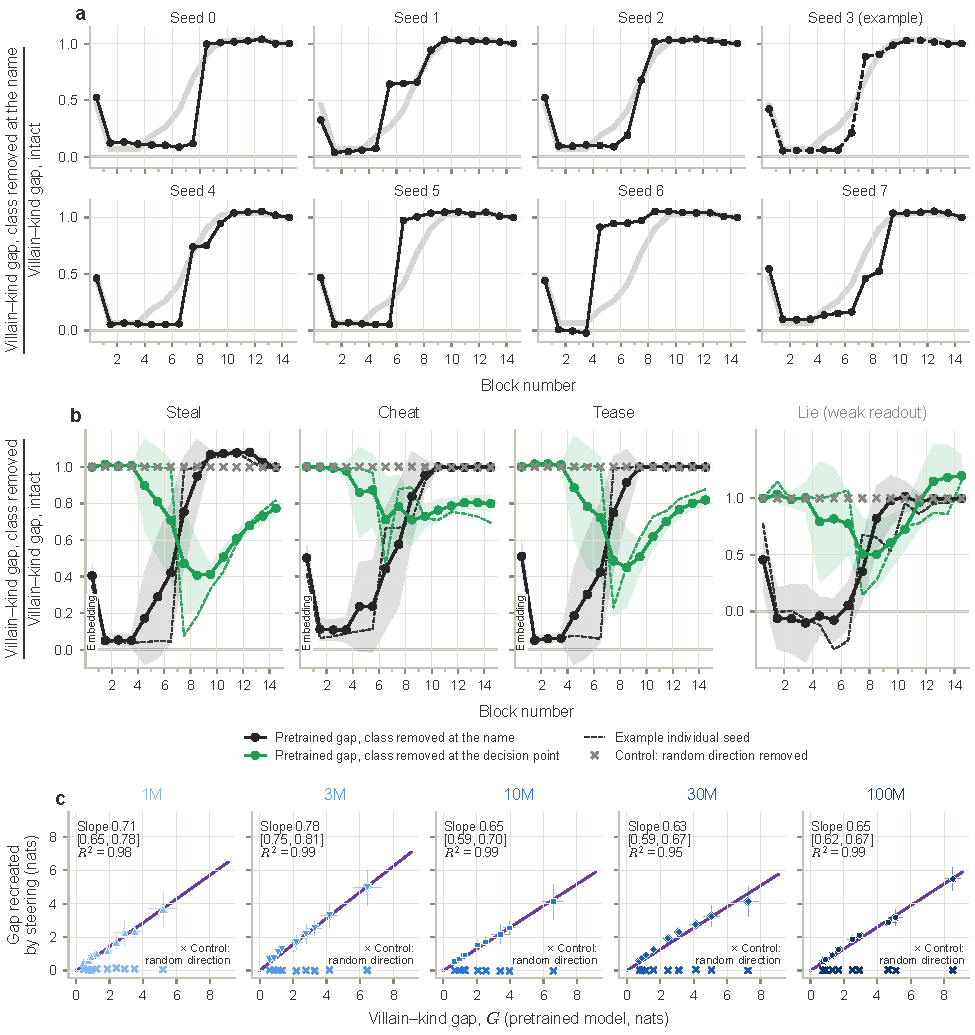
\includegraphics[width=\textwidth]{figA3_flow_by_act.pdf}
  \caption{
    \textbf{Interventions on activations, separated by seed, act, and model size.}
    We split out aggregated plots from \cref{fig:mechanism} for reference.
    \panel{a} See \cref{fig:mechanism}b, specifically the pretrained gap with the class removed at the name.
    Gray: mean over seeds (as plotted in \cref{fig:mechanism}b).
    Black: each individual seed. We chose seed 3 (dashed) as a representative example in \textbf{b} and \cref{fig:mechanism}b (see text).
    \panel{b} See \cref{fig:mechanism}b, which was averaged over all four acts.
    Here, we plot them separately.
    Note wider y range for ``lie'' due to the broader confidence intervals.
    Pretrained gap only (no finetunes shown).
    \panel{c} See \cref{fig:mechanism}c. Here we split the data into separate plots for each model size, including separate linear fits through the origin.
    Under the slope annotation, we list 95\% CI for the slopes and $R^2$ from regression.
  }
  \label{fig:flowbyact}
\end{figure}
